\documentclass[11pt, letterpaper, titlepage]{article}
\usepackage[utf8]{inputenc}
\usepackage[export]{adjustbox}
\usepackage{geometry}
 \geometry{
 a4paper,
 total={168mm,257mm},
 left=20mm,
 top=15mm,
 includefoot,includehead
 }



\usepackage[backend=biber, style=authoryear, giveninits=true, maxbibnames=25, uniquename=init, maxcitenames=2, hyperref=true, dashed=false]{biblatex}			% Benutze Biber/BibLaTeX zum Zitieren
\addbibresource{main.bib}					% Pfad zur BibTeX Datei aus Citavi
\renewcommand{\cite}{\parencite}
\usepackage{caption}
\usepackage{subcaption}
\usepackage{graphicx}
\usepackage{svg}
\usepackage{placeins}
\usepackage[hidelinks]{hyperref}
\usepackage{amsmath}
\usepackage[headsepline]{scrlayer-scrpage}
\clearpairofpagestyles %Seitenzahl nicht in der Kopfzeile
\usepackage{acronym}

\title{MeetEU Project - Team Heidelberg - Team 1 -- \\ Identification and Enhancement of novel Sars-CoV-2 NSP13 helicase inhibitors}
\author{Linda Blaier, Paul Brunner, Selina Ernst, Valerie Segatz and Chlo\'{e} Weiler}
\date{February 2024}

\begin{document}

\maketitle

\ihead{\headmark}
\automark{section}  %Kopfzeile gleich dem Sektiontitel
\cfoot{\pagemark}   %\ofood Seitenzahl rechts

\section{Abstract}
One of the most important factors in ending the Covid-19 pandemic was the quick development of a working vaccine. However, the treatment options for acute Covid-19 infections are still limited. One possibility to accelerate the development of new therapies is to screen already approved or well understood compounds for effects against the viral reproduction. In this years MeetEU project, we investigated the NSP13 helicase of Sars-CoV-2 and tried to find compounds that could be repurposed for this therapy, as well as novel compounds that could lead to an effective treatment of Covid-19. Due to its central part in the viral replication and the conservation of its sequence, it is a prime target for drug development. We were able to provide an \textit{in-silico} pipeline (Figure \ref{workflow}) to screen compound databases and extract compounds, which could possibly be used as a therapeutic against Covid-19. A binding pocket was established as the consensus of three different tools. Using AutoDock Vina and Glide we scanned FDA approved drugs, as well as well-understood biological compounds for how well they bind in the binding pocket. Additionally, we evaluated the toxicity of the compounds to make choosing a lead for drug development easier. After validation of the top scoring compounds using DiffDock and Molecular Dynamics Simulation, the identified drug leads could be used for wet-lab research. \\
\begin{figure}[h]
  \centering
  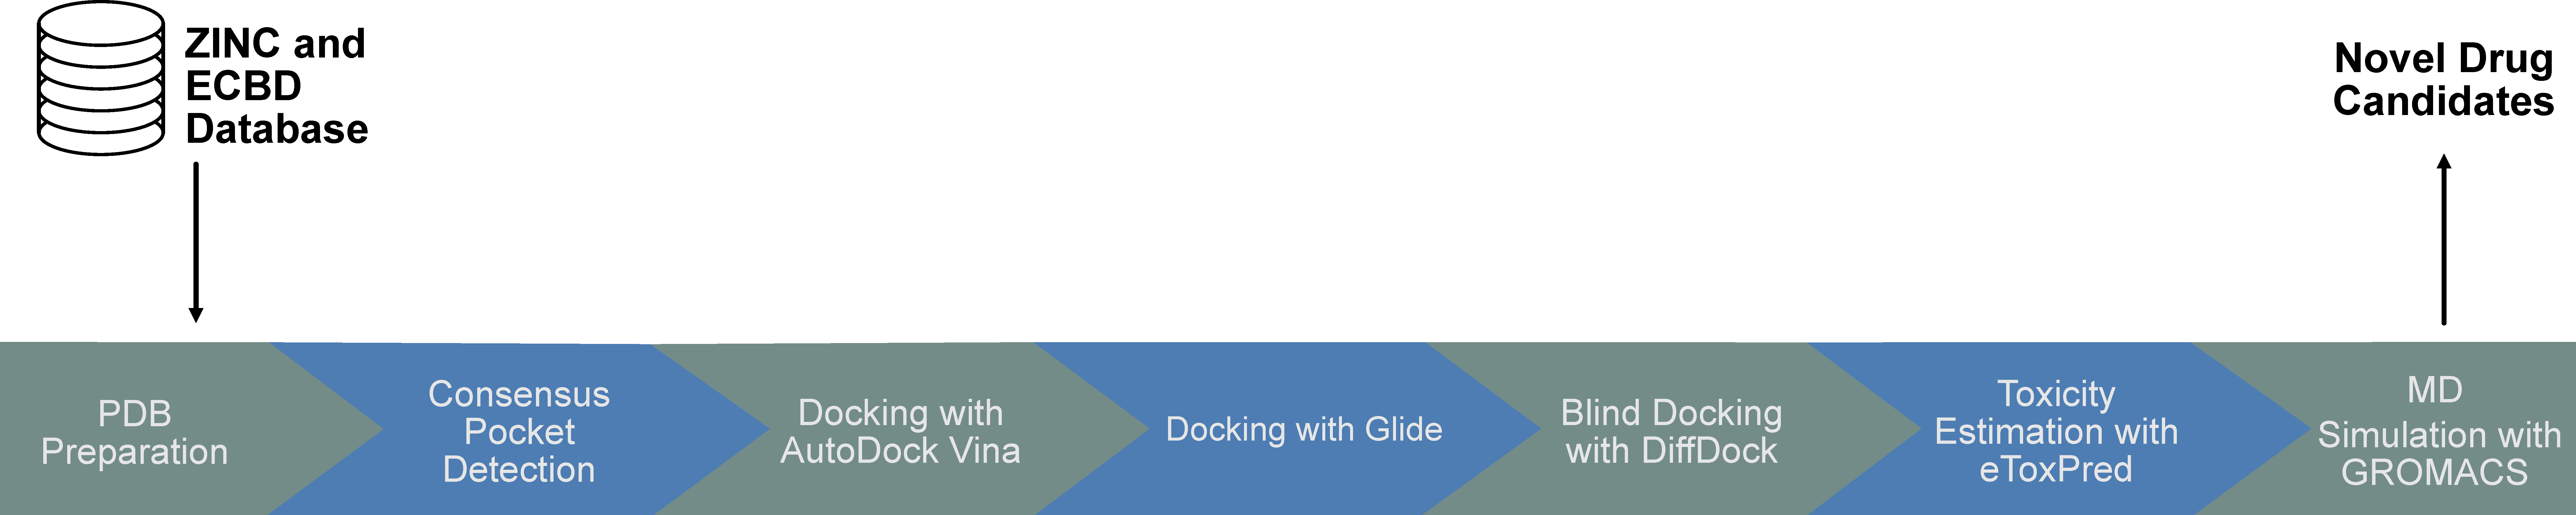
\includegraphics[width=\textwidth]{Workflow_MeetEU.pdf}
  \caption{Proposed workflow for the discovery and improvement of NSP13 helicase inhibitors.}
  \label{workflow}
\end{figure}
\newpage
\FloatBarrier
%    Abkürzungsverzeichnis
{\setlength{\parskip}{0.2cm}
\section*{Abbreviations}
    \begin{acronym}[LC-MS/MS23]
        % A B C D E F G H I J K L M N O P Q R S T U V W X Y Z        
        % Abkürzungen
        \acro{MD}{molecular dynamics}
        \acro{NSP13}{non-structural protein 13}
        \acro{RMSD}{root-mean square deviation}
        \acro{RMSF}{root-mean square fluctuation}
        \acro{MM-PBSA}{molecular mechanics energies combined with the Poisson-Boltzmann and surface area continuum solvation}
        % Formelzeichen
        
        
        % als benutzt markierte Acronyme    
        
        
    \end{acronym}
}
\newpage

\section{Introduction}
Even though the development of vaccines against Sars-CoV-2 was successful during the recent pandemic, the amount of FDA approved drugs for the therapy of Covid-19 is still limited to Paxlovid and Veklury, Olumiant and Actemra \cite{FDACOVID}. As vaccines are not able to prevent 100\% of infections, enhancing the landscape of possible drugs used to treat Covid-19 would especially benefit people at risk of a harsh pathogenesis. The goal of this years Meet-EU project was to investigate the \ac{NSP13} helicase of the Sars-CoV-2 virus for possible vulnerabilities to inhibitors. The helicase is strongly conserved between corona viruses, and thus offers a nice target for drugs, as it is less likely for the drugs to become ineffective due to rapid changes in the viral genome. In general \ac{NSP13} is a vital component of the viral replication mechanism and thus inhibiting it would severely hinder the spread of the virus in the host. The protein consists of five domains, namely the zinc binding domain, the stalk domain, as well as 1A, 2A and 1B. The latter three make up the catalytic centre of the protein, where RNA and ATP bind \cite{NSP13_basics}. \\
In order to explore possible new therapy options it makes sense to perform an \textit{in-silico} screening of different compounds to identify groups of compounds that interact well with the NSP13 helicase. This screening process involves several steps: Identify possible binding sites, screen ligands for how well they bind in this pocket and validate the findings to generate a suggestion, as to which compounds would be worth it to investigate in a wet-lab setting. Focussing this screening on well documented or already FDA approved compounds significantly simplifies a potential registration of a potential new drug entering the market. 
%\subsection{Lead Drug Enhancement}
%In order to enhance the binding affinity of our drug candidates and thus their performance, we used AutoGrow4 (Version 4.0.3) \cite{packageAutogrow4} to generate novel compounds. Starting with the best binding compounds of our initial docking simulation with AutoDock Vina as generation zero, multiple new structures are generated by combining sub-structures of the first generation or by passing them through a set of possible chemical reactions after converting them into their respective SMILES codes. All of the generated compounds are ranked by their binding affinity. After passing several filters the best performing compounds are used as the seed for the next generation. Using this algorithm, compounds are found, which show higher binding affinities than the first generation. As AutoGrow4 labels all new structures by the path by which they were obtained, we can also evaluate the synthesizability.  

\subsection{Molecular Dynamics Simulation}
As the last step of our pipeline, an \ac{MD} simulation is conducted using the best scoring compounds as a ligand in the binding pocket of the NSP13 protein. Simulating the movement of molecules in a system based on the attracting and repulsing forces between atoms helps us a lot with understanding the molecular interplay between the ligands found and the binding pocket. Whether the ligand stays inside of the binding pocket throughout the whole simulation gives an estimate on how strongly it binds to the protein \cite{MD_Basics}. As this is the final step of our pipeline, the result of this simulation estimates how the ligand would perform if applied \textit{in-vitro}. Additionally, the frames generated by the software can be used to calculate different metrices regarding the binding strength, like the \ac{RMSF}, \ac{RMSD} and the binding affinities estimated by \ac{MM-PBSA}. The \ac{RMSD} measures the average displacement of the atoms throughout the simulation compared to the first frame of the simulation and estimates how much the protein moves and changes conformations over time. The \ac{RMSF} on the other hand calculates the movement of a certain atom or group of atoms over time compared to the average position of the atoms and groups \cite{RMSD_RMSF}. \ac{MM-PBSA} is able to estimate the binding affinity of the simulated protein-ligand pair \cite{MM_PBSA}.


\section{Material and Methods}
\subsection{Datasets from ZINC20 and ECBL}
A total of 1616 fda approved drugs were downloaded in .sdf format from the ZINC database \cite{Irwin.2020}. Additional, 5016 fiels were retrieved, downloading the pilot library from the ECBL database.

\subsection{Receptor and ligand preparation}
Ligands were prepared using openbable in order to convert implicit hydrogens into explicit hydrogens, generate necessary 3D structures of the ligands, as well as to split mulitmolecule files into single ones. ADFR suite was further used in order to convert all files into the .pdbqt format, which is required by Autodock Vina. 
 
%\subsection{Generation of novel structures}
%Using the same PDB file of the nsp13 A-chain, the top 10 best scoring drugs from our initial AutoDock Vina docking were passed to AutoGrow4 (Version 4.0.3 \textcite{packageAutogrow4}) as SMILES. The docker container provided by the package maintainers was used, as it guarantees no problems concerning version incompatibilities. Using a similar configuration to what \Citeauthor{packageAutogrow4} used for lead drug improvement, AutoGrow4 generated and re-scored a plethora of novel structures. Due to our limited amount of structures in generation zero, we opted to disable the generation of cross-over molecules for the first generation. The configuration file can be found in the appendix. As we try to improve a small amount of lead drugs, AutoGrow4 generates many new molecules per generation, while it is only run for five generations. This enables us to explore different modifications to our compounds while not making synthesis too complicated, as there is a maximum of five modifications happening. Because AutoGrow4 also enables structures with a diverse structure to pass into next generations even though they might not be top performers yet, we can be sure to explore a vast landscape of different possible drugs.

\subsection{Molecular Dynamics Simulation}
In order to validate the binding of the discovered compounds, we used GROMACS (Version 2023.3, \textcite{packageGROMACS}) to simulate the drugs inside of the ATP binding site of NSP13. To do so, the Protein-Ligand Complex tutorial by \Citeauthor{Lemkul2018} was followed \cite{Lemkul2018}. The a99SB-disp forcefield was used, as it was shown to recreate protein structures in different environments very accurately \cite{Forcefield}. The 6ZSL PDB file was first turned into the fitting GROMACS format (\textit{.gro}). Using the \textit{.gro} file, the general simulation parameters are set up. This includes setting the size and shape of the simulation box, which was set to be a dodecahedron in this case. \\ 
As the ligands feature bonds and atoms not commonly seen in proteins, it is required to create a fitting force-field for them. For this, acpype \cite{acpype} was used, which was developed to be compatible with AMBER force-fields. The output files from Maestro Glide were converted to PDB and then piped into acpype. The software uses the given PDB file and information about the charges on the compound to create multiple files for different simulation suites, that enable us to add the compound to the simulation environment with the right descriptions of its atoms.  The output of acpype was then combined with the GROMACS topology and \textit{.gro} files manually, according to \Citeauthor{Lemkul2018}. \\
Following the tutorial, the simulation space was created, filled with water (a99SBdisp\_water used as its force-field) and ions were added to create a net zero charge system. As it is common the charges were equalized using sodium and chloride ions. Energy-minimization was conducted and \textit{NVT} and \textit{NPT} equilibration was used to finish the simulation setup. The V-Rescale thermostat was used for thermal coupling in the \textit{NVT} equilibration and for the \textit{NPT} equilibration, a Parrinello-Rahman pressure coupling was used. This ensures a somewhat stable starting point for the simulation. For these steps, the protein and ligand were energetically coupled, as they are in close proximity to each other. The rest of the simulation space, namely ions and water, were also coupled. The production run was set to simulate 100 ns, using a Leap-Frog Integrator. The \textit{.mdp} file containing the simulation parameters used for the final production run can be seen in the appendix. One of these runs took approximately  36 h, which was made possible by parallelization and usage of a NVIDIA V100 GPU. \\ 
For the analysis of the simulation, GROMACS internal tools were used to calculate the RMSD and RMSF of the protein. These scores give us insight into the movement and conformational changes during the simulation regarding protein and ligand. Furthermore, the simulation frames were extracted and rendered into a video using VMD \cite{VMD}. For MM-PBSA calculations we used gmx\_MMPBSA \cite{MMPBSA1}. This package enables direct calculation of binding affinities using the GROMACS output files.
\section{Results} 
\subsection{Molecular dynamics simulation validates binding of top scorers}
The \ac{MD} simulation is an integral part to validate the results of our pipeline. After the production run was finished, the resulting trajectory file was centered on the protein and modified to remove any ghosting and splitting of the protein at the borders of the simulation box. The last frame of the simulation was extracted and visualized using pyMOL \cite{PyMOL}, which can be seen in Figure \ref{MD.Annotated}. 
\begin{figure}[h]
  \begin{center}
    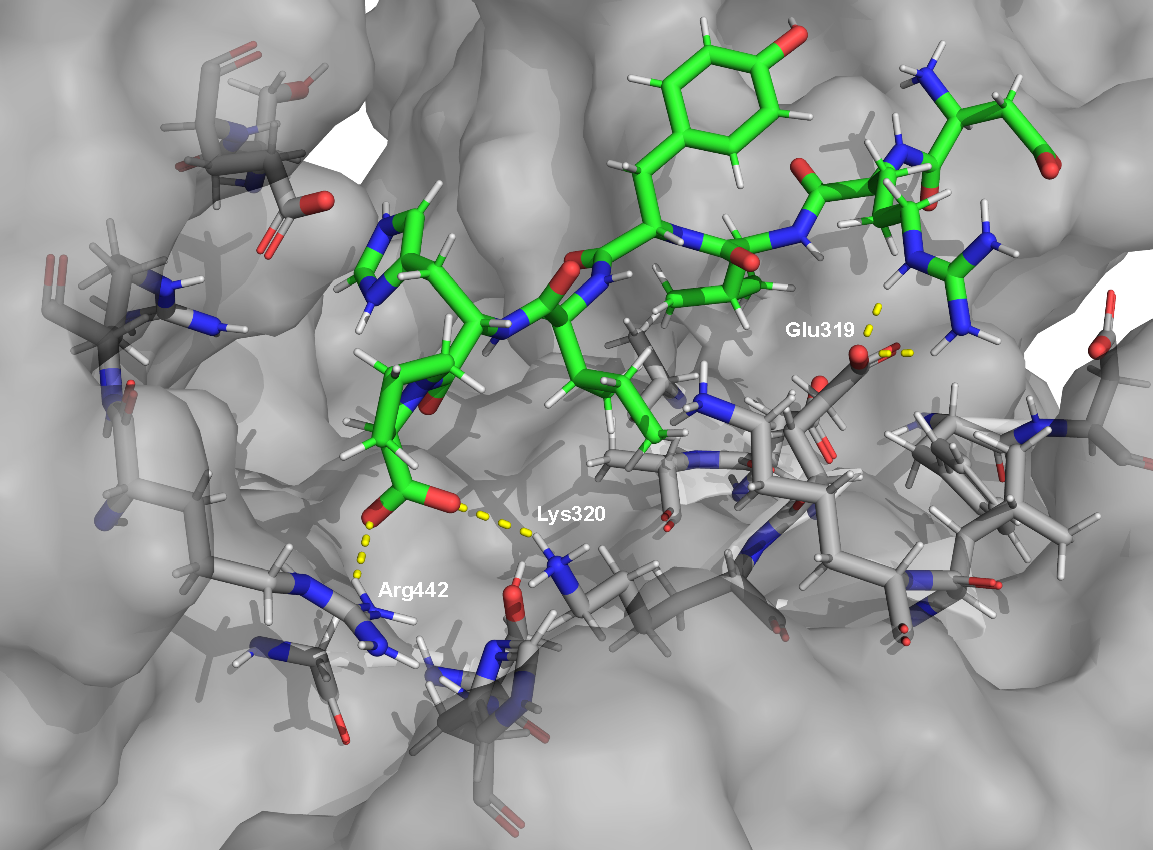
\includegraphics[width=0.9\textwidth]{last_frame_render_annotated.pdf}
  \end{center}
  \caption{\textbf{Visualisation of EOS100380 inside the binding pocket at the end of 100 ns simulation.} The polar interactions are marked with yellow dotted lines. The amino acids involved in these interactions are labelled.}\label{MD.Annotated}
\end{figure}

The figure clearly demonstrated, that the top scoring compound of our Glide screening stayed inside of the binding pocket until the end of the simulation. Furthermore, the polar interactions between the ligand and residues in its proximity is shown. It seems, that EOS100380 is bound to the protein by interactions with Glu319, Lys320 and Arg442 of the NSP13 helicase. These interactions could also be validated by LigPlot+ \cite{LigPlot}. \\

To investigate the dynamics of these interactions between ligand and protein, the \ac{RMSD} and \ac{RMSF} were calculated, which can be obeserved in Figure~\ref{rms}. 
\begin{figure}[h]
  \begin{center}
    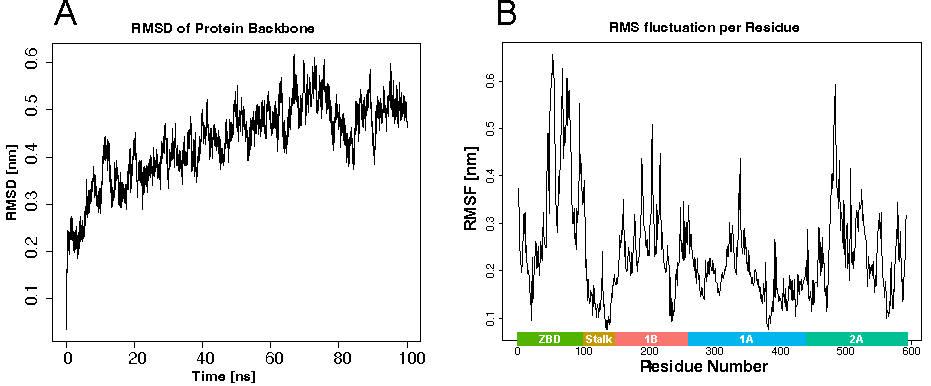
\includegraphics[width=1.0\textwidth]{RMS_Protein.pdf}
  \end{center}
  \caption{\textbf{RMSD and RMSF of the protein backbone during the simulation.} The RMSD was plotted over time for the whole 100 ns simulation. The RMSF is shown per residue. The colorbar annotates the protein domain the respective residue belongs to, according to \textcite{Domains}. ZBD = zinc binding domain}
  \label{rms}
\end{figure}
The \ac{RMSD} observed over the course of the simulation (Figure~\ref{rms}A) rises at first, but reaches a plateau after roughly 60 ns. The RMSD seems to settle at roughly 0.5 nm, which is slightly larger than expected. Investigation into the RMSF per residue (Figure~\ref{rms}B) suggests, that some residues move significantly more than others. The highly mobile atoms seem to be located in the zinc binding domain and domains 1B and 2A, which both play a role in the binding of the ligand. Thus movement in these parts of the protein was to be expected. All in all, the protein seems to undergo conformational changes, however it does not show major signs of instability. 


\FloatBarrier

\section{Discussion and Outlook}

\section{Supplementary Material}

\pagebreak
\FloatBarrier

\renewcommand{\bibname}{References}  % damit Literatuverzeicnis mit "References" betitelt
\printbibliography


\end{document}
